\documentclass{article}

\usepackage[fontsize=11.0pt]{fontsize}
\usepackage{times}
\usepackage[T1]{fontenc}
\usepackage[square,sort,comma,numbers]{natbib}
\bibliographystyle{abbrvnat}

\usepackage[margin=0.85in]{geometry}
\setlength{\parskip}{4pt}
\setlength{\parindent}{0pt}
\usepackage[compact]{titlesec}

\usepackage{enumitem}
\usepackage{url}
\usepackage{graphicx}
\usepackage{booktabs}
\usepackage{subcaption}
\usepackage{placeins}
\setlength{\floatsep}{8pt plus 2pt minus 2pt}
\setlength{\textfloatsep}{10pt plus 2pt minus 2pt}
\usepackage{hyperref}
\hypersetup{colorlinks=true, linkcolor=blue, citecolor=blue, urlcolor=blue}

\usepackage{mathtools, amsmath, amssymb}
\usepackage{titling}

%----------------------------------------------------------------------------------------
\begin{document}

\begin{flushleft}
\textbf{\Large Modelling Single-cell RNA-Seq Data Distributions:\\
Evaluating Zero-Inflation in UMI Count Data} \\[6pt]
CPSC 445 (Algorithms in Bioinformatics) Course Project \\
Submitted April 13, 2026; revised September 2026.\footnote{\raggedright The analysis, code, and figures are unchanged. The revision also corrects several statements against the archived pipeline outputs, including one rounding error in Table~\ref{tab:percluster} (see the README). The submitted version is tagged \texttt{submitted-2026-04-13} at \url{https://github.com/Redtropig/scrna-zero-inflation}.}
\end{flushleft}

%----------------------------------------------------------------------------------------
\begin{abstract}
Single-cell RNA sequencing (scRNA-seq) generates sparse count matrices that are challenging to model statistically.
A long-standing debate concerns whether the observed excess of zeros in these data reflects genuine ``zero-inflation'' requiring specialized distributions, or is simply a consequence of cell-type heterogeneity, cell-to-cell differences in sequencing depth, and low capture efficiency.
In this project, we fit four count distributions to \emph{all} 9{,}107 post-QC genes (mean UMI $>$ 0.01) of the PBMC 3k dataset: Poisson, Negative Binomial (NB), Zero-Inflated Poisson (ZIP), and Zero-Inflated Negative Binomial (ZINB).
We use all genes rather than the standard subset of highly variable genes, which is circularly biased toward overdispersed models, and we measure the size of that bias.
Each fit is performed both with and without a per-cell log-library-size offset, which shows how much of the apparent overdispersion is explained by depth heterogeneity alone.
The comparison connects directly to the multinomial view of UMI counts of Townes et al.~\cite{townes2019feature}.
With the offset included, Bayesian Information Criterion (BIC) model selection assigns the simple Poisson distribution to 56.2\% of genes in the pooled analysis, NB to 39.8\%, and flags only 0.3\% of genes as zero-inflated; the stratification by expression decile shows that the Poisson regime dominates low-expression genes while NB remains the appropriate model at the high-expression tail.
After further conditioning on cell type via Leiden clustering, Poisson dominance rises further and zero-inflation evidence stays negligible.
We corroborate these findings with two deep generative models: scVI~\cite{lopez2018deep} trained under ZINB, NB, and Poisson likelihoods, and GLM-PCA~\cite{townes2019feature} trained under explicit multinomial, Poisson, and NB likelihoods.
Both confirm that overdispersion modelling matters far more than zero-inflation modelling, and that the multinomial perspective on UMI counts is indistinguishable from a per-cell-offset Poisson in practice.
Our results show that, for UMI-based droplet scRNA-seq, choosing the right observation family is primarily about library-size correction and cell-type conditioning, not zero inflation.
\end{abstract}

%----------------------------------------------------------------------------------------
\section{Introduction}

Single-cell RNA sequencing (scRNA-seq) enables transcriptome-wide profiling at single-cell resolution.
A fundamental challenge in analyzing scRNA-seq data is choosing an appropriate statistical model for the count matrices, which are characteristically sparse.
For a typical gene, often more than 90\% of entries are zero.

The question of whether these zeros reflect a ``zero-inflated'' data-generating process has been one of the most debated topics in the field.
Early methods, including ZIFA~\cite{pierson2015zifa}, explicitly assumed zero-inflation and modelled scRNA-seq data with zero-inflated distributions that posit two distinct mechanisms for generating zeros: ``structural'' zeros (from dropout events or true biological absence) and ``sampling'' zeros (from the count distribution itself).
This led to the widespread adoption of the Zero-Inflated Negative Binomial (ZINB) distribution in tools such as scVI~\cite{lopez2018deep} and ZINB-WaVE~\cite{risso2018general}.

However, a series of influential papers challenged this assumption.
Svensson~\cite{svensson2020droplet} demonstrated that in droplet-based scRNA-seq data with unique molecular identifiers (UMIs), the observed number of zeros is consistent with standard count distributions (Poisson or Negative Binomial) without any zero-inflation component.
Because UMIs eliminate PCR amplification bias, simple sampling models describe the data well.
Kim et al.~\cite{kim2020demystifying} showed that most apparent ``drop-outs'' vanish once cell-type heterogeneity is resolved through clustering, suggesting that imputation or zero-inflation modelling is unnecessary and potentially harmful.
Pan et al.~\cite{pan2023poisson} further demonstrated that an independent Poisson distribution fits UMI-based scRNA-seq data well, with each gene in each cell following a Poisson with a very small rate parameter for the many zeros.

Choi et al.~\cite{choi2020bayesian} applied Bayesian model selection and found statistical evidence of zero-inflation in some datasets, but attributed it to biological factors (cell type, sex) rather than technical artifacts.
Despite finding zero-inflation, they recommended the standard Negative Binomial as the reference model for scRNA-seq analysis, as ZINB parameter estimates are unreliable indicators of true zero-inflation.
A comprehensive review by Jiang et al.~\cite{jiang2022statistics} synthesized this debate, noting that the critical distinction is not droplet-based versus plate-based technology, but rather the use of UMIs.

In this project, we compare four count distributions (Poisson, NB, ZIP, and ZINB) on the PBMC 3k benchmark dataset, with three design choices that address issues we believe are common in the literature.
First, we fit \emph{all} post-QC genes rather than only the top highly variable genes (HVGs), the subset our proposal had planned to use.
Feedback on the proposal pointed out that this subset is circular.
HVG selection (Seurat v3 variance-stabilizing transformation) preferentially picks genes whose variance exceeds the empirical mean-variance trend (i.e., genes that are overdispersed), so running a Poisson-vs-NB contest on HVGs alone is pre-biased toward NB and overstates the apparent dominance of overdispersed models.
Second, every fit is performed under a per-cell log-library-size offset $\log s_i$ in addition to a classical no-offset baseline.
This is equivalent, under a Poisson likelihood, to a multinomial likelihood conditional on each cell's total count~\cite{townes2019feature}, and it lets us quantify how much of the pooled overdispersion is simply a consequence of cell-to-cell depth differences.
Third, we complement scVI's three observation likelihoods with GLM-PCA~\cite{townes2019feature}, whose ``mult'' family is an explicit multinomial approximation and whose ``poi'' and ``nb'' families let us triangulate the scVI conclusions on a different latent-variable backbone.
With these three choices, we reproduce the core messages of Svensson~\cite{svensson2020droplet}, Kim et al.~\cite{kim2020demystifying}, and Pan et al.~\cite{pan2023poisson} on the full gene set and with explicit depth correction.

%----------------------------------------------------------------------------------------
\section{Methods}

\subsection{Dataset and Preprocessing}

We used the PBMC 3k dataset from 10x Genomics, accessed via the Scanpy library~\cite{wolf2018scanpy}.
This dataset contains peripheral blood mononuclear cells from a healthy donor, profiled using the 10x Chromium platform with UMI-based counting.
After quality control (filtering cells with fewer than 200 or 5{,}000 or more detected genes, removing cells with $\geq$10\% mitochondrial reads, and filtering genes detected in fewer than 3 cells), we retained 2{,}694 cells and 13{,}712 genes.

Raw UMI counts were preserved in an AnnData layer for distribution fitting.
For clustering \emph{only}, we normalized counts to 10{,}000 per cell, log-transformed, selected the top 2{,}000 highly variable genes (HVGs) using the Seurat v3 method, and performed PCA (50 components), followed by neighbour graph construction (10 nearest neighbours, 40 principal components) and UMAP embedding.
Leiden clustering at resolution 1.0 identified 10 clusters, which were annotated to 8 cell types using canonical marker genes (e.g., CD14/LYZ for monocytes, CD79A for B cells, NKG7 for NK cells).
HVG selection is used only for the clustering front-end and for the scVI and GLM-PCA training inputs.
All per-gene distribution fitting uses the full set of 9{,}107 post-QC genes whose mean UMI count exceeds 0.01, to avoid the circular bias described in the Introduction.

\subsection{Size Factors and the Multinomial Connection}
\label{sec:sizefactors}

For every cell $i$ we define a size factor $s_i = T_i / \widetilde{T}$ where $T_i$ is the cell's total UMI count and $\widetilde T$ is the median total count across cells.
When included as an offset $\log s_i$ in a Poisson GLM with an intercept-only linear predictor for each gene $j$,
\[
X_{ij}\sim\text{Poisson}(s_i\mu_j),
\]
the resulting likelihood factorizes as a product of independent Poissons.
The gene-level MLE is
\[
\hat\mu_j = \frac{\sum_i X_{ij}}{\sum_i s_i},
\]
and the per-cell row-sums are a sufficient statistic for $s_i$.
Conditional on those row-sums, the joint distribution of the counts of a single cell across genes is exactly multinomial in the gene proportions~\cite{townes2019feature}.
We therefore treat the Poisson-with-offset fit as an \emph{empirical realization} of the multinomial view of scRNA-seq data, and contrast it directly with the no-offset fit, where cell-to-cell depth differences are instead absorbed into the dispersion parameter of an NB.

\subsection{Statistical Distributions}

We compared four count distributions. In all four, the per-cell mean is allowed to scale with $s_i$ when the log-offset is used, giving the parameterizations:

\textbf{Poisson} (1 gene-level parameter, $\mu_j$):
$X_{ij}\sim \mathrm{Poisson}(s_i\mu_j)$; $\text{Var}(X_{ij}) = \mathrm{E}[X_{ij}] = s_i\mu_j$.

\textbf{Negative Binomial} (2 parameters, $\mu_j, \phi_j$):
mean $s_i\mu_j$, variance $s_i\mu_j + (s_i\mu_j)^2/\phi_j$; as $\phi_j\to\infty$, NB collapses to Poisson.

\textbf{Zero-Inflated Poisson} (2 parameters, $\pi_{0j}, \mu_j$):
$P(X_{ij}=0) = \pi_{0j} + (1-\pi_{0j})e^{-s_i\mu_j}$.

\textbf{Zero-Inflated Negative Binomial} (3 parameters, $\pi_{0j}, \mu_j, \phi_j$):
NB count component with a Bernoulli zero-inflation probability $\pi_{0j}$.

Setting $s_i\equiv 1$ for all cells recovers the no-offset fits we report for the ablation.

\subsection{Parameter Estimation}

For \textbf{Poisson}, the offset-aware MLE has a closed form: $\hat\mu_j = \sum_i X_{ij}/\sum_i s_i$ (with $s_i\equiv 1$ in the no-offset baseline).
For \textbf{NB}, we use a profile-likelihood scheme: given a trial $\phi$, we solve the score equation $\sum_i \phi(X_{ij}-s_i\mu)/(s_i\mu+\phi)=0$ for $\mu$ by Newton iteration, and refine $\phi$ via bounded Brent search over $\log\phi$.
For \textbf{ZIP} and \textbf{ZINB}, we call \texttt{statsmodels}' \texttt{ZeroInflatedPoisson} and \texttt{ZeroInflatedNegativeBinomialP} with an intercept-only design, a logit inflate link, and the same $\log s_i$ offset; convergence defaults to BFGS with a Nelder-Mead fallback.
All per-gene fits are parallelized across $N-1$ CPU cores via \texttt{joblib.Parallel}.
A synthetic sanity test verifies on \mbox{$X_i\sim\text{Poisson}(s_i\cdot 2)$} with $s_i\sim U(0.2,3)$ that the offset pathway drives the NB dispersion $\phi$ from 3.4 (without offset) to 104 (with offset), and recovers $\hat\mu=2.03$.

\subsection{Model Selection}

For each gene, we computed the Bayesian Information Criterion:
$\text{BIC} = k \ln(n) - 2 \ln(\hat{L})$,
where $k$ is the number of parameters, $n$ is the sample size, and $\hat{L}$ is the maximized likelihood.
Lower BIC indicates a better model, balancing fit against complexity.
We also computed $\Delta\text{BIC}$, the difference between the best non-ZI and best ZI model; a gene is classified as ``zero-inflated'' if $\Delta\text{BIC} > 10$ (very strong evidence on the Kass-Raftery scale~\cite{kass1995bayes}).

\subsection{Heterogeneity Analysis}

To test whether apparent zero-inflation and overdispersion are artifacts of mixing cell types, we repeated the entire fitting and model selection pipeline \emph{within} each Leiden cluster (cell type), restricting to clusters with $\geq$50 cells and to genes whose within-cluster mean count still exceeds 0.01.
Within each cluster we recompute cell-specific size factors against that cluster's own median total count, so the depth correction remains unit-median locally.
This follows the logic of Kim et al.~\cite{kim2020demystifying}: if zeros are caused by cell-type heterogeneity (a gene is ``ON'' in some cell types and ``OFF'' in others), then within a homogeneous population and after depth correction, the simpler Poisson model should suffice~\cite{pan2023poisson}.

\subsection{scVI Deep Generative Model Comparison}

We trained three scVI models~\cite{lopez2018deep} on the 2{,}000 HVGs with \texttt{gene\_likelihood} set to \texttt{zinb}, \texttt{nb}, and \texttt{poisson}, respectively.
All models used 10 latent dimensions, 128 hidden units, 1 layer, and were trained for up to 200 epochs with 90/10 train/validation split and early stopping (patience=10).
We compared models using: (1) importance-weighted marginal log-likelihood, (2) UMAP embeddings of the latent spaces, and (3) posterior predictive checks comparing per-gene zero fractions, means, and variances between real and simulated data.
scVI internally estimates a per-cell latent library-size variable $\ell_i$, so its likelihoods are already size-aware; our univariate analysis above uses the classical $\log s_i$ offset for the same reason.

\subsection{GLM-PCA Multinomial Comparison}

Because scVI does not ship a multinomial observation likelihood, we additionally fit GLM-PCA~\cite{townes2019feature} with three families: \texttt{mult} (an explicit binomial approximation to the multinomial), \texttt{poi}, and \texttt{nb}.
GLM-PCA uses the same HVG input matrix as scVI and a matching latent dimensionality of ten, optimized by Fisher scoring with $L_2$ penalty 1 for up to 200 iterations.
We evaluate each family by (i) final training deviance, (ii) adjusted Rand index (ARI) and normalized mutual information (NMI) between Leiden clusters recomputed on the GLM-PCA factors and the cell-type labels derived from the log-normalized HVG PCA, and (iii) UMAP layouts.

%----------------------------------------------------------------------------------------
\section{Results}

\subsection{Dataset Characteristics}

Figure~\ref{fig:overview} shows the PBMC 3k dataset after preprocessing.
The UMAP embedding reveals distinct cell-type clusters spanning CD4 T, CD14$^+$ monocytes, B cells, CD8 T, NK, FCGR3A$^+$ monocytes, dendritic cells, and platelets.
Total UMI counts per cell span roughly an order of magnitude, and FCGR3A$^+$ monocytes and dendritic cells have substantially higher totals than lymphocytes.
The analysis below depends on this depth heterogeneity.

\begin{figure}[!htbp]
\centering
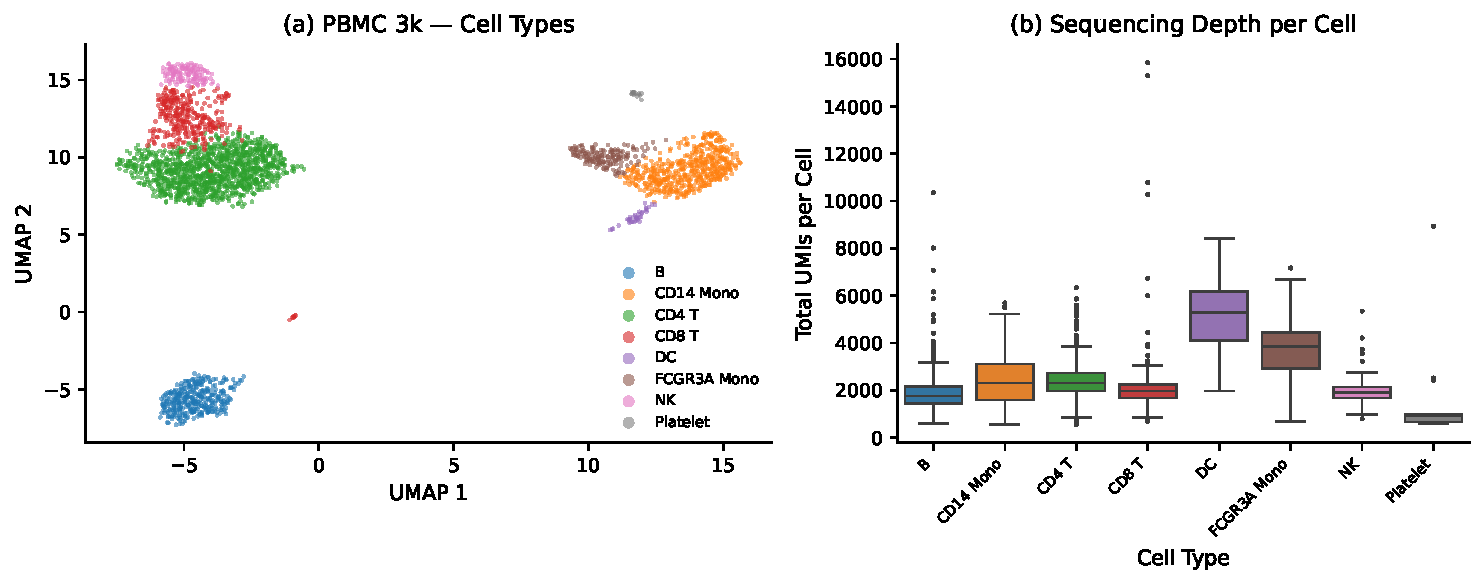
\includegraphics[width=\textwidth]{data/figures/fig1_dataset_overview.pdf}
\caption{PBMC 3k dataset overview. (a) UMAP embedding coloured by annotated cell type. (b) Distribution of total UMI counts per cell across cell types; note the order-of-magnitude spread.}
\label{fig:overview}
\end{figure}

\subsection{HVG Bias and Library-Size Offset Ablation}

Of the top 2{,}000 HVGs, 1{,}719 pass the mean filter.
On these genes alone, the no-offset fits select the Negative Binomial by BIC for 99.1\% of them, with Poisson never winning.
That result reflects two choices in the setup, which the next two paragraphs change one at a time.

\textbf{All-gene fitting.}
When the contest is re-run on the \emph{full} set of 9{,}107 post-QC genes but still without an offset, Poisson already wins for 51.9\% of genes and NB for 43.6\% (ZIP 4.2\%, ZINB 0.2\%).
The reversal occurs because HVG selection, by construction, picks genes whose variance exceeds the empirical mean-variance trend, so a Poisson-vs-NB BIC contest on HVGs alone is biased against Poisson from the start.
This re-run still treats cells as exchangeable, and still recovers the Kass--Raftery ``barely any zero-inflation'' verdict: only 9/9{,}107 genes (0.1\%) are flagged at $\Delta\text{BIC}>10$.

\textbf{Library-size offset.}
Adding a per-cell $\log s_i$ offset to every fit shifts a further $\sim$4 percentage points of winners from NB into Poisson: Poisson rises to 56.2\%, NB falls to 39.8\%, ZIP to 3.5\%, ZINB to 0.5\%, and $\Delta\text{BIC}>10$ flags 30/9{,}107 genes (0.3\%).
The residual NB dominance concentrates at the high-expression tail, where true biological variability remains the limiting source of dispersion even after depth correction (see the decile stratification in Figure~\ref{fig:decile}).
All four distributions converge on 100\% of fits in both modes.
Figure~\ref{fig:ablation} summarizes the ablation.

\begin{figure}[!htbp]
\centering
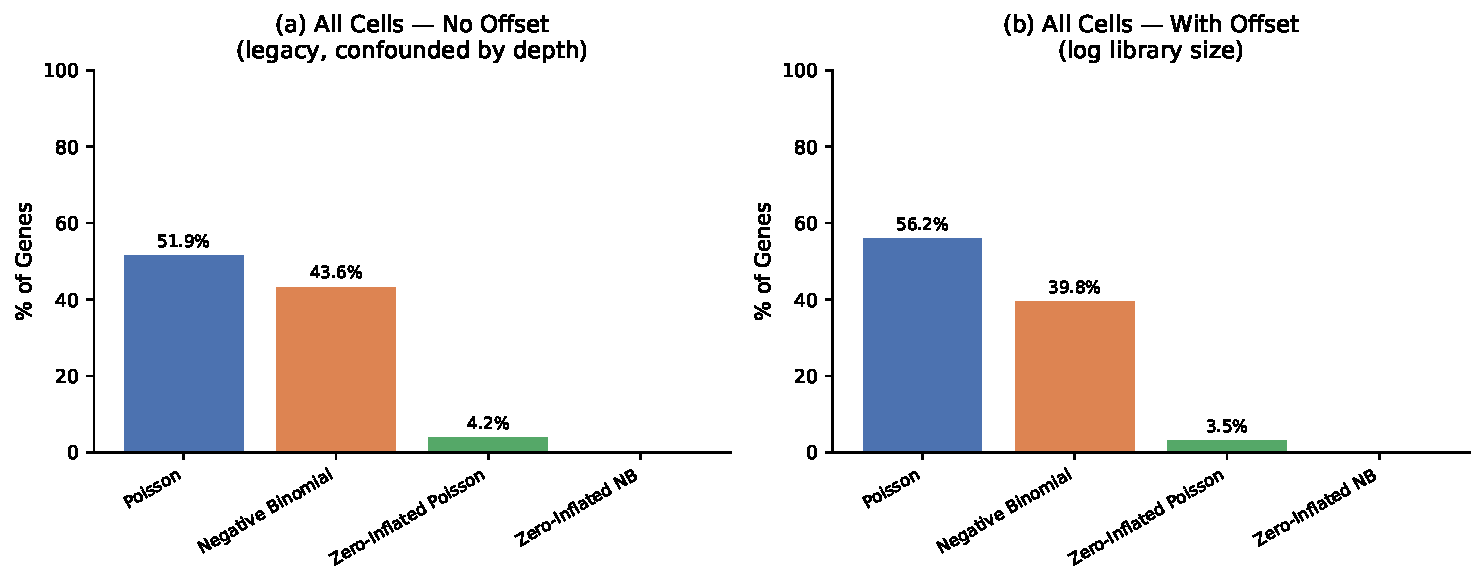
\includegraphics[width=\textwidth]{data/figures/fig2_offset_ablation.pdf}
\caption{All-cells BIC model selection on the complete 9{,}107-gene set. (a) No library-size offset. (b) With $\log s_i$ offset. Adding the offset shifts a further $\sim$4 percentage points of winners from NB to Poisson.}
\label{fig:ablation}
\end{figure}

\textbf{Where in the expression spectrum does each distribution dominate?}
Figure~\ref{fig:decile} shows the offset-aware BIC winners stratified by gene-mean decile.
Low-expression genes (deciles 1--4) are overwhelmingly Poisson; across the middle deciles (5--7) Poisson's lead narrows until NB overtakes it at decile 7; and the top two deciles are dominated by NB.
The Poisson--NB variance law predicts this pattern: NB only begins to outperform Poisson on BIC once $\mu^2/\phi$ overtakes sampling noise, which in practice happens only for the genes with high enough means.

\begin{figure}[!htbp]
\centering
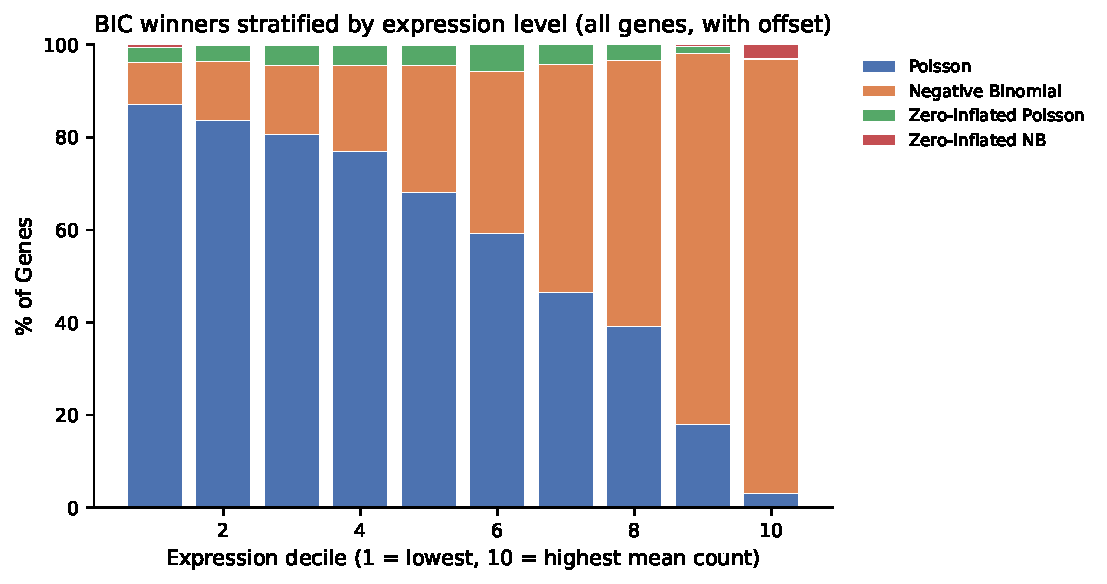
\includegraphics[width=\textwidth]{data/figures/fig3_by_expression.pdf}
\caption{Offset-aware BIC winners stratified by gene-expression decile. Poisson dominates low-expression genes; NB dominates the high-expression tail; ZI models remain a small minority at every expression level.}
\label{fig:decile}
\end{figure}

\textbf{Zero-fraction calibration and mean--variance structure} are shown in Figure~\ref{fig:diag}: offset-aware NB zero-fraction predictions track the $y=x$ diagonal cleanly across the full dynamic range, confirming that depth-corrected NB adequately explains the zeros without needing a zero-inflation component.

\begin{figure}[!htbp]
\centering
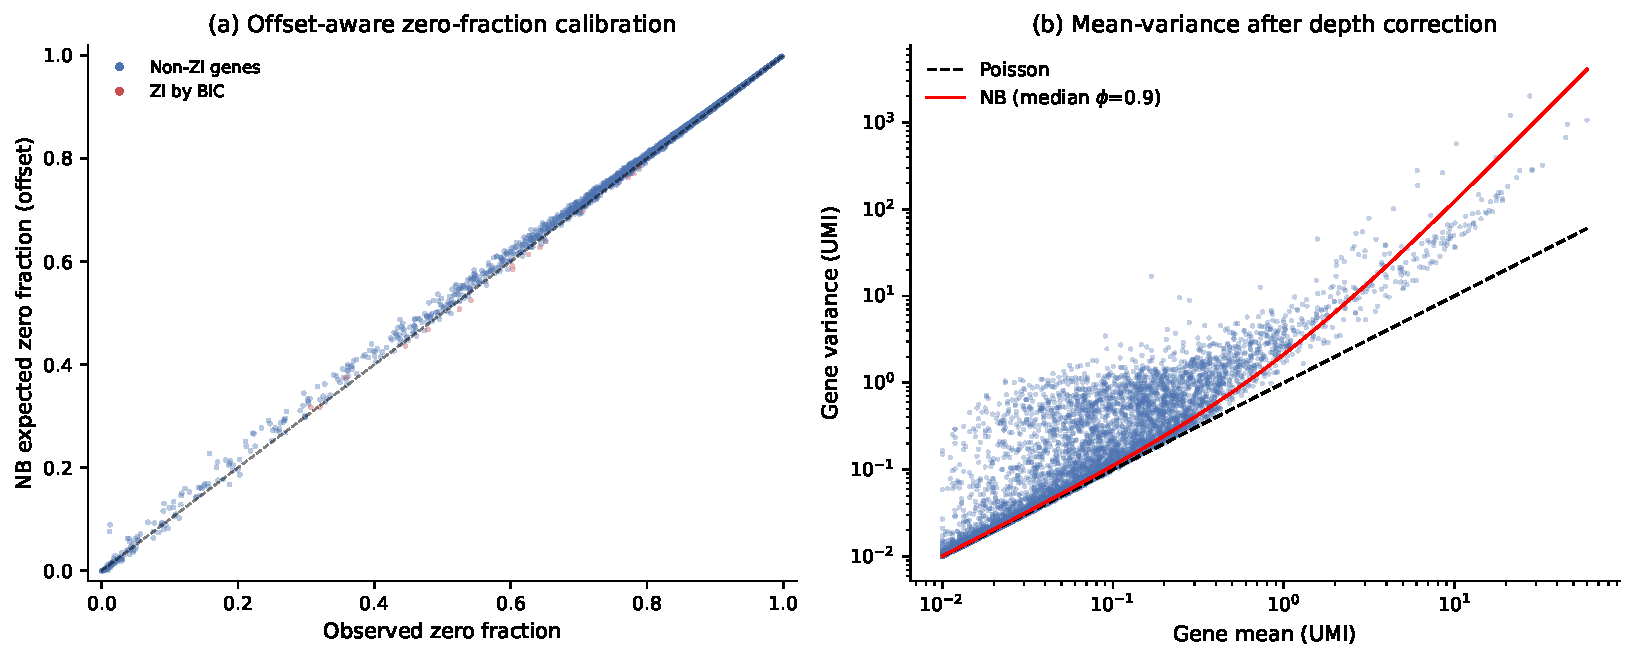
\includegraphics[width=\textwidth]{data/figures/fig4_diagnostics.pdf}
\caption{(a) Observed vs.\ offset-aware NB-expected zero fractions. Red points are the few genes flagged as zero-inflated. (b) Mean-variance plot with Poisson reference (dashed) and NB reference curve at median $\phi$.}
\label{fig:diag}
\end{figure}

\subsection{Effect of Cell-Type Conditioning}

Restricting the fit to cells within a single Leiden cluster and re-computing size factors locally further increases Poisson dominance (Figure~\ref{fig:het}).
This reproduces the central conclusion of Kim et al.~\cite{kim2020demystifying} and Pan et al.~\cite{pan2023poisson} on our expanded gene set and with library-size correction: after conditioning on cell type and sequencing depth, the count process is essentially Poisson for the overwhelming majority of genes, zero-inflation is vanishingly rare, and what residual NB there is sits at the high-expression tail.
Table~\ref{tab:percluster} gives the BIC winner percentages for all four combinations of cell grouping and offset mode.

\begin{figure}[!htbp]
\centering
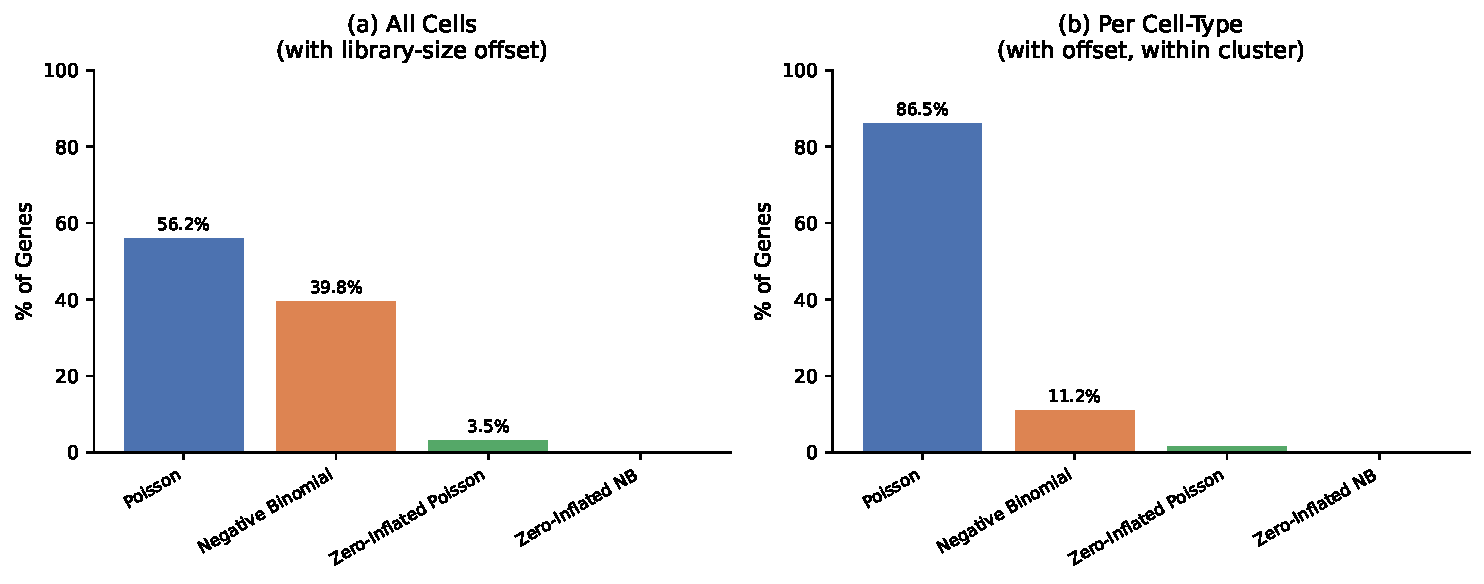
\includegraphics[width=\textwidth]{data/figures/fig5_heterogeneity.pdf}
\caption{BIC model selection: all cells (with offset) vs per cell-type cluster (with offset). Conditioning on cell type substantially increases Poisson dominance (56.2\%~$\to$~86.5\%), while residual zero-inflation remains negligible ($\leq$0.4\% at both levels).}
\label{fig:het}
\end{figure}

\begin{table}[!htbp]
\centering
\caption{BIC winner percentages across analysis modes, comparing all-cells and per-cluster fits under both offset settings.}
\label{tab:percluster}
\begin{tabular}{lccccc}
\toprule
Source & \%Poisson & \%NB & \%ZIP & \%ZINB & $\Delta$BIC$>$10 \\
\midrule
All cells (offset)      & 56.2 & 39.8 & 3.5 & 0.5 & 0.3\% \\
Per cell-type (offset)  & 86.5 & 11.2 & 1.9 & 0.4 & 0.3\% \\
Per cell-type (no off.) & 85.1 & 12.4 & 2.3 & 0.2 & 0.1\% \\
All cells (no offset)   & 51.9 & 43.6 & 4.2 & 0.2 & 0.1\% \\
\bottomrule
\end{tabular}
\end{table}

\subsection{scVI Deep Generative Model Comparison}

Table~\ref{tab:scvi} summarizes the scVI results across three observation likelihoods.
The scVI models handle library size internally through a per-cell latent variable $\ell_i$, so they need no external offset.

\begin{table}[!htbp]
\centering
\caption{scVI model comparison. Marginal LL is the importance-weighted marginal log-likelihood (higher is better). PPC correlations measure agreement between real and simulated data statistics.}
\label{tab:scvi}
\begin{tabular}{lcccc}
\toprule
Likelihood & Marginal LL & PPC Zero-Frac $r$ & PPC Mean $r$ & PPC Var $r$ \\
\midrule
ZINB    & $-616.9$ & 0.995 & 0.991 & 0.982 \\
NB      & $-627.3$ & 0.996 & 0.998 & 0.888 \\
Poisson & $-677.7$ & 0.997 & 0.997 & 0.985 \\
\bottomrule
\end{tabular}
\end{table}

\textbf{Marginal log-likelihood}: ZINB achieves the best marginal log-likelihood ($-616.9$), followed by NB ($-627.3$) and Poisson ($-677.7$).
The gap between ZINB and NB ($\sim$10 nats per cell) is modest compared to the NB--Poisson gap ($\sim$50 nats per cell), indicating that overdispersion modelling matters much more than zero-inflation modelling.
The univariate analysis above points the same way.

\textbf{Latent spaces and PPCs} (Figures~\ref{fig:scvi}--\ref{fig:ppc}): All three scVI variants produce qualitatively similar UMAP embeddings with clear cell-type separation; the NB model shows the lowest variance correlation (0.888) in the posterior-predictive check, while ZINB and Poisson both exceed 0.98.

\begin{figure}[!htbp]
\centering
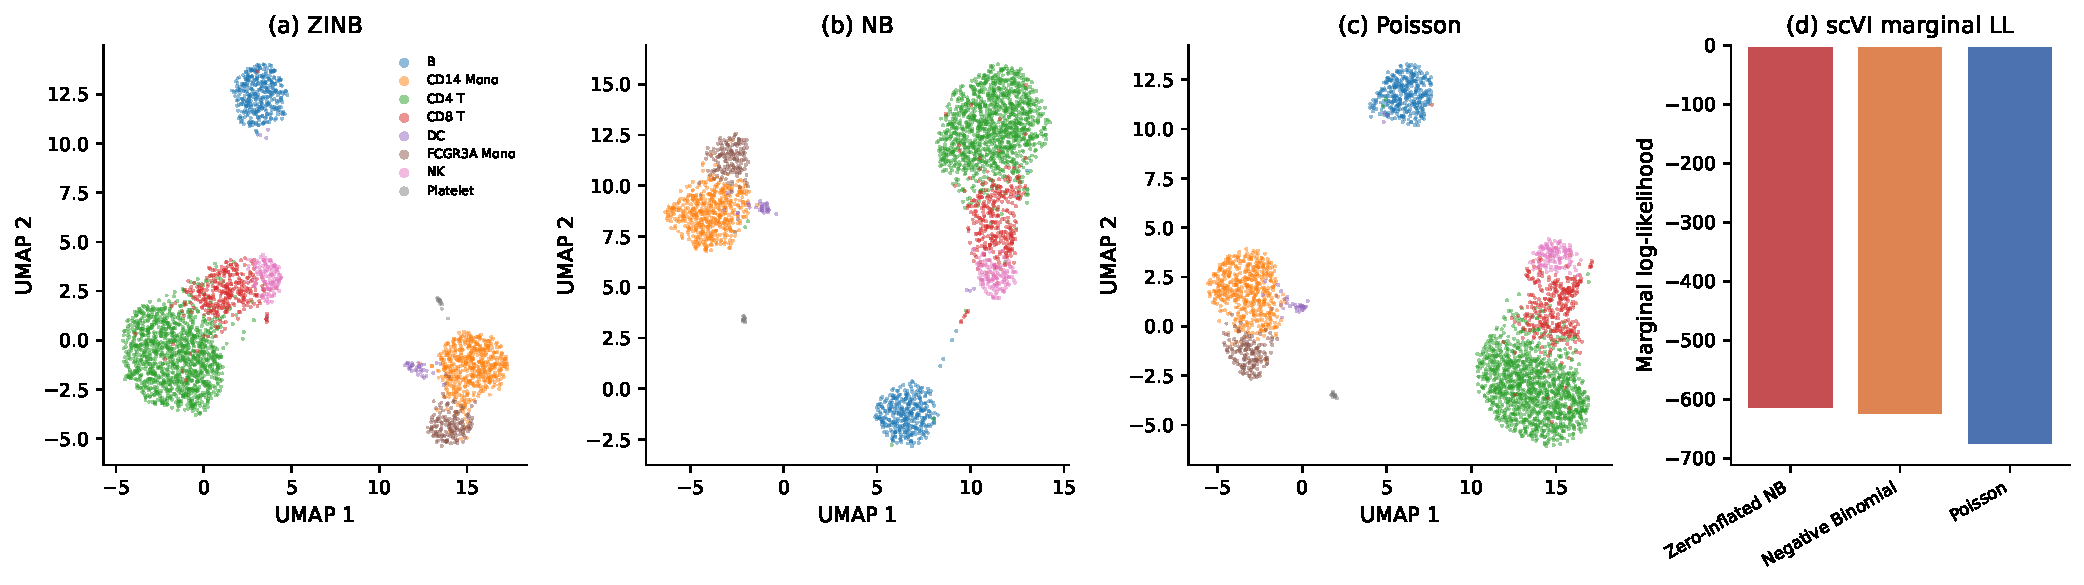
\includegraphics[width=\textwidth]{data/figures/fig6_scvi_comparison.pdf}
\caption{scVI comparison. (a--c) UMAP embeddings of latent spaces from ZINB, NB, and Poisson models, coloured by cell type. (d) Marginal log-likelihoods.}
\label{fig:scvi}
\end{figure}

\begin{figure}[!htbp]
\centering
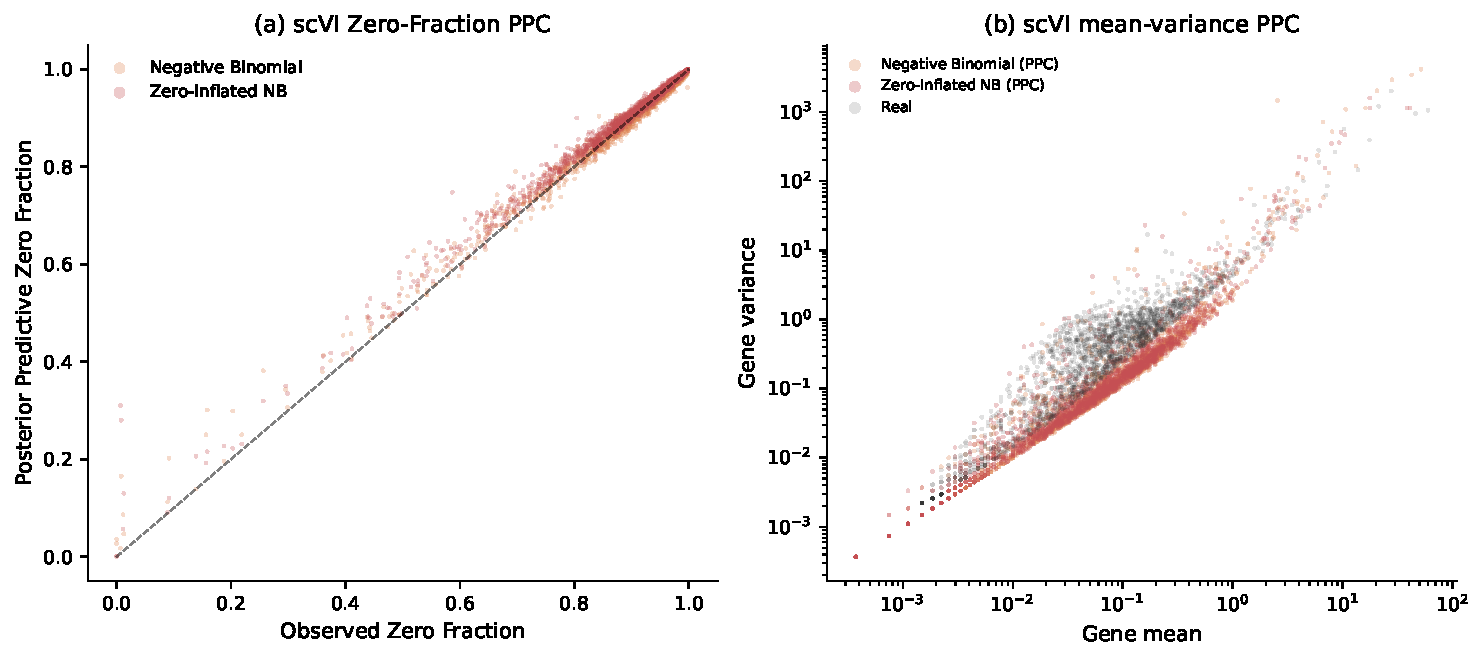
\includegraphics[width=\textwidth]{data/figures/fig7_ppc.pdf}
\caption{Posterior predictive checks. (a) Observed vs.\ simulated zero fractions for NB and ZINB scVI models. (b) Mean-variance relationship in simulated vs.\ real data.}
\label{fig:ppc}
\end{figure}

\subsection{GLM-PCA: An Explicit Multinomial Comparator}

Table~\ref{tab:glmpca} compares the three GLM-PCA families (\texttt{mult}, \texttt{poi}, and \texttt{nb}), fitted on the same HVG input matrix and latent dimensionality as scVI.

The NB family achieves the lowest final deviance ($1.68\times10^6$) compared to Poisson ($2.39\times10^6$) and multinomial ($2.40\times10^6$), consistent with the scVI marginal-LL ranking.
Clustering quality, however, is much closer across families: the Poisson and NB families yield similar ARI (0.500 vs.\ 0.533) and NMI (0.714 vs.\ 0.728) against the annotated cell types, and multinomial falls between them (ARI 0.501, NMI 0.723).
The Poisson and multinomial deviances differ by only 0.2\%, consistent with the Poisson--multinomial equivalence of Section~\ref{sec:sizefactors}, and their downstream ARIs are nearly identical (0.501 vs.\ 0.500), which supports the practical equivalence of the two likelihoods.
The small remaining deviance gap is plausibly due to the binomial approximation used by the \texttt{mult} family (see Limitations).
The NB family's lower deviance buys almost no improvement in downstream clustering, mirroring the scVI pattern where overdispersion modelling helps fit quality but not biological discovery.
Figure~\ref{fig:glmpca} shows the UMAP layouts and ARI comparison across the three families.

\begin{table}[!htbp]
\centering
\caption{GLM-PCA comparison across three likelihood families (10 latent dimensions, 200 max iterations, $L_2$ penalty 1).}
\label{tab:glmpca}
\begin{tabular}{lrrrr}
\toprule
Family & Final Deviance & ARI & NMI & Runtime (s) \\
\midrule
Multinomial & $2.40\times10^6$ & 0.501 & 0.723 & 88 \\
Poisson     & $2.39\times10^6$ & 0.500 & 0.714 & 50 \\
Neg.\ Binomial & $1.68\times10^6$ & 0.533 & 0.728 & 191 \\
\bottomrule
\end{tabular}
\end{table}

\begin{figure}[!htbp]
\centering
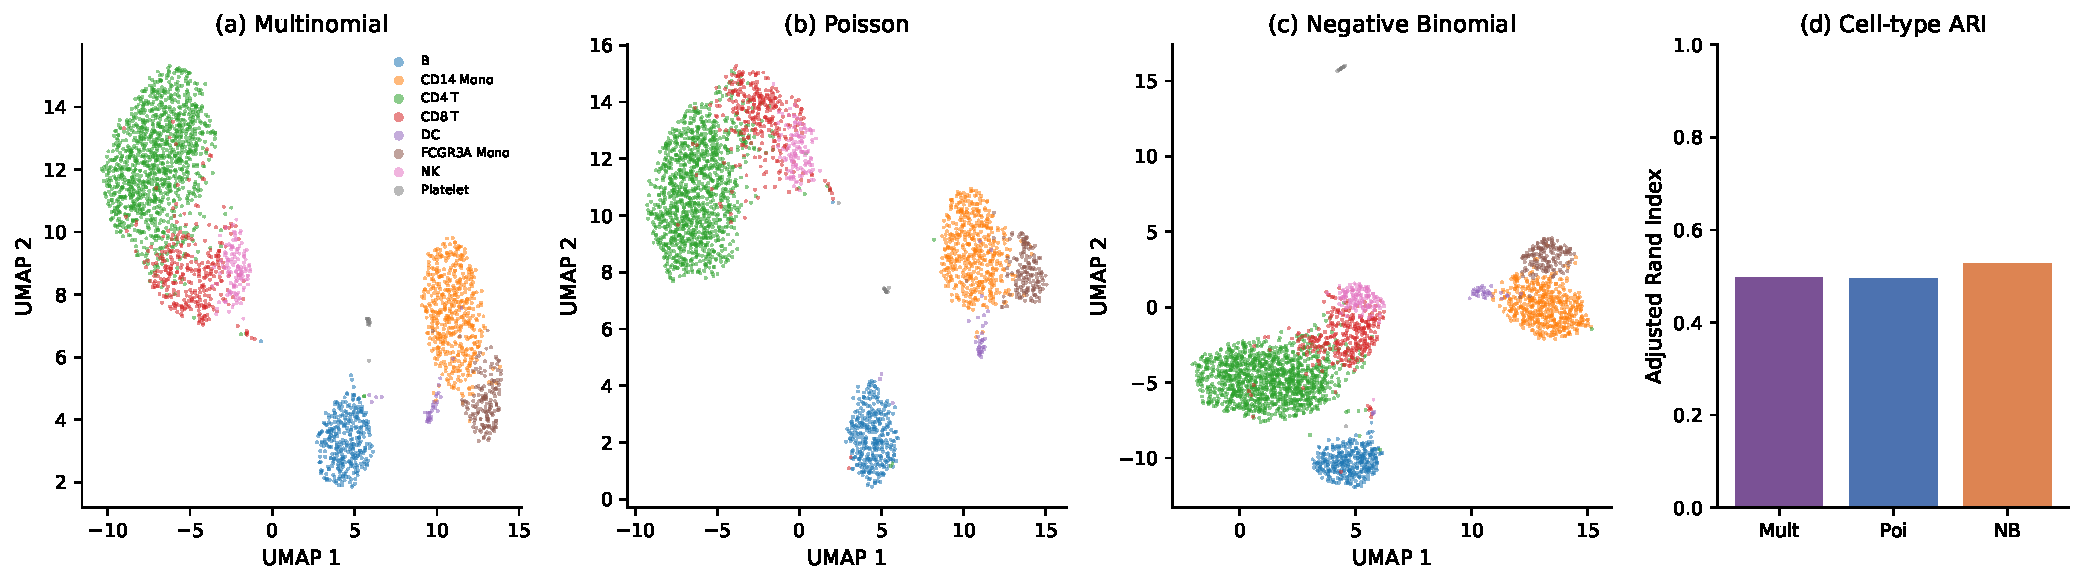
\includegraphics[width=\textwidth]{data/figures/fig8_glmpca.pdf}
\caption{GLM-PCA comparison under (a) multinomial, (b) Poisson, and (c) NB likelihoods. (d) Adjusted Rand Index between Leiden clustering on the GLM-PCA factors and the annotated cell-type labels.}
\label{fig:glmpca}
\end{figure}

%----------------------------------------------------------------------------------------
\FloatBarrier
\section{Discussion}

\subsection{Summary of Findings}

Our analysis yields five findings for UMI-based scRNA-seq data:

\begin{enumerate}[nosep]
\item \textbf{HVG bias inflates NB dominance.}
  Restricting the fits to the HVGs selected by Seurat v3 gives NB as the BIC winner for $>$99\% of genes.
  The result is circular, since HVG selection preferentially picks genes whose variance exceeds the empirical mean-variance trend.
  On the full 9{,}107-gene set \emph{without} offset, Poisson already wins 51.9\% of genes and NB falls to 43.6\%.

\item \textbf{Library-size offset further shifts the balance.}
  Adding a per-cell $\log s_i$ offset moves another $\sim$4 pp from NB to Poisson (56.2\% vs.\ 39.8\%), confirming that a substantial fraction of apparent overdispersion comes from differences in sequencing depth rather than biological variance.

\item \textbf{Cell-type conditioning makes the Poisson regime dominant.}
  Within Leiden clusters, Poisson wins 86.5\% of 58{,}614 gene--cluster BIC contests (with offset), NB 11.2\%, and only 0.3\% of pairs are flagged as zero-inflated ($\Delta\text{BIC}>10$).
  This reproduces the core message of Kim et al.~\cite{kim2020demystifying} and Pan et al.~\cite{pan2023poisson} on an expanded gene set with explicit depth correction.

\item \textbf{Zero-inflation is negligible throughout.}
  In every analysis reported here, no more than 0.4\% of tests reach the $\Delta\text{BIC}>10$ threshold, confirming Svensson~\cite{svensson2020droplet}.

\item \textbf{Deep generative and latent-variable models concur.}
  scVI ranks ZINB $>$ NB $\gg$ Poisson on marginal log-likelihood, but the ZINB--NB gap ($\sim$10 nats/cell) is modest next to the NB--Poisson gap ($\sim$50 nats/cell), so modelling overdispersion matters far more than modelling zero-inflation.
  GLM-PCA's Poisson and multinomial families differ by only 0.2\% in deviance and give nearly identical clustering ARI (0.501 vs.\ 0.500), consistent with the theoretical Poisson--multinomial equivalence.
\end{enumerate}

\subsection{Implications for Practitioners}

\textbf{Model choice.}
For UMI-based data, NB remains a safe default for pooled analyses because it absorbs both biological variance and residual depth effects.
However, practitioners should be aware that most of its advantage over Poisson disappears once (a) a library-size offset is included and (b) cell types are resolved.
Zero-inflated models add complexity without meaningful improvement at any analysis level, consistent with Choi et al.~\cite{choi2020bayesian}.

\textbf{Cluster, then model.}
Following Kim et al.~\cite{kim2020demystifying}, clustering should precede distribution-dependent analyses such as differential expression testing.
Within clusters and after depth correction, the simple Poisson is the appropriate default for the vast majority of genes; NB is needed only for the high-expression tail where biological dispersion is detectable.

\textbf{scVI and GLM-PCA likelihood.}
When using scVI, \texttt{gene\_likelihood="nb"} is recommended over the default ZINB for UMI data, as it reduces model complexity without sacrificing performance.
For GLM-PCA, the Poisson and multinomial families are interchangeable in practice and both are faster than NB.

\subsection{Limitations}

\begin{itemize}[nosep]
\item \textbf{Single dataset.}
  We analyzed only the PBMC 3k dataset.  While PBMCs are a standard benchmark, results may differ for other tissues, organisms, or larger cell counts.

\item \textbf{UMI-only conclusions.}
  Our findings apply to UMI-based droplet protocols (10x Chromium).  Non-UMI technologies (Smart-seq2) may genuinely exhibit zero-inflation due to PCR amplification bias~\cite{jiang2022statistics}.

\item \textbf{Intercept-only ZI models.}
  We used intercept-only models for ZIP/ZINB, assuming a gene-global zero-inflation probability.  Gene-by-cell or covariate-dependent ZI models might uncover structured zero-inflation that our tests miss.

\item \textbf{GLM-PCA multinomial approximation.}
  The \texttt{mult} family in GLM-PCA uses a binomial approximation to the multinomial, not the exact multinomial likelihood; in practice the approximation is tight for the gene proportions observed here, but may diverge on datasets with fewer genes or more dominant transcripts.

\item \textbf{Cluster resolution dependence.}
  Per-cluster results depend on the Leiden resolution parameter and therefore on the granularity of cell-type definition.  A finer or coarser resolution could shift the Poisson/NB balance within clusters.
\end{itemize}

\subsection{Connection to the Literature}

Our results are consistent with the review by Jiang et al.~\cite{jiang2022statistics}, which identifies the use of UMIs, not the technology platform, as the critical factor.
UMIs effectively eliminate PCR amplification bias, making the data well-described by simple sampling models.
For modern UMI-based protocols, the ``zero-inflation controversy'' is largely resolved.
The zeros are expected under NB (or Poisson within cell types) and do not require specialized modelling.
Beyond reproducing these conclusions, our analysis measures the HVG selection bias and the effect of a library-size offset, and compares Poisson and multinomial likelihoods directly with GLM-PCA~\cite{townes2019feature}.

%----------------------------------------------------------------------------------------
\bibliography{ref}
\end{document}
